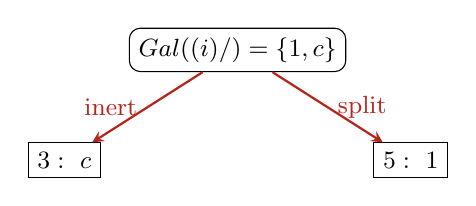
\begin{tikzpicture}[>=stealth,font=\small]
\node[draw,rounded corners] (a) at (0,0) {$\operatorname{Gal}(\Q(i)/\Q)=\{1,c\}$};
\node[draw] (b) at (-2.2,-1.4) {$3:\ c$};
\node[draw] (c) at (2.2,-1.4) {$5:\ 1$};
\draw[->,BrickRed,thick] (a)--node[left] {inert}(b);
\draw[->,BrickRed,thick] (a)--node[right] {split}(c);
\end{tikzpicture}
